% Header: General study / work / project template
%%%%%%%%%%%%%%%%%%%%%%%%%%%%%%%%%%%%%%%%%%%%%%%%%%%%%%%%%%%%%%%%%%%

\documentclass[11pt,a4paper]{scrartcl}

% Layout
\usepackage[margin=2.5cm]{geometry}
\usepackage[onehalfspacing]{setspace}

% General packages
\usepackage{graphicx}
\usepackage{enumitem}
\usepackage{tcolorbox}
\tcbuselibrary{breakable}
\usepackage[breaklinks=true,colorlinks=true,linkcolor=blue,urlcolor=blue,citecolor=blue]{hyperref}
\usepackage{amsmath,amsthm,amssymb,mathtools}
\usepackage{icomma}
\usepackage[T1]{fontenc}
\usepackage[utf8]{inputenc}

% Language: choose one
% \usepackage[ngerman]{babel}
\usepackage[english]{babel}

% Units / tables / floats / references
\usepackage[locale = UK,space-before-unit=true,per-mode = symbol]{siunitx}
\usepackage{booktabs,multirow}
\usepackage{placeins}
\usepackage[natbib,abbreviate=true,doi=false,style=numeric-comp,giveninits=true,sorting=none]{biblatex}
\usepackage{csquotes}

% Optional bibliography
% \addbibresource{references.bib}

% Graphics paths
\graphicspath{{Bilder/} {images/} {figures/} {chapters/}}

% Optional math shortcuts
\newcommand{\R}{\mathbb{R}}
\newcommand{\N}{\mathbb{N}}
\newcommand{\Q}{\mathbb{Q}}
\newcommand{\set}[1]{\left\{ #1 \right\}}
\newcommand{\abs}[1]{\left| #1 \right|}
\newcommand{\norm}[1]{\left\lVert #1 \right\rVert}
\newcommand{\ol}[1]{\overline{#1}}

% Optional units
\DeclareSIUnit{\dBm}{dBm}

% Box styles
\newtcolorbox{calculationbox}[1][]{
    title=Calculation,
    breakable,
    #1
}

\newtcolorbox{solutionbox}[1][]{
    title=Solution,
    breakable,
    #1
}

\newtcolorbox{answerbox}[1][]{
    title=Answer,
    breakable,
    #1
}

\newtcolorbox{notebox}[1][]{
    title=Notes,
    breakable,
    #1
}

\newtcolorbox{sidecalcbox}[1][]{
    title=Side Calculation,
    breakable,
    #1
}

%%%%%%%%%%%%%%%%%%%%%%%%%%%%%%%%%%%%%%%%%%%%%%%%%%%%%%%%%%%%%%%%%%%
\begin{document}

\title{Physik 4 - Blatt 03}
\author{Tobias Laser}
\date{\today}
\maketitle
\vfill
\thispagestyle{empty}

\pagenumbering{arabic}

\paragraph{Aufgabe 1: Teilchenbeschleuniger}

\begin{enumerate}[label=(\alph*)]
    \item Der $3.2$ km lange Linearbeschleuniger (ein HF-Linearbeschleuniger) am SLAC arbeitet mit einer Beschleunigungsspannung von $250$ kV. Welche Elektronenenergie konnte er dann ursprünglich mit Hilfe von ca. $100000$ Driftröhren erreichen? 
    \begin{calculationbox}
        $E_{kin} = N \cdot q \cdot U = 10^5 \cdot e \cdot 250 \cdot 10^3 \text{V} = 25$ MeV
    \end{calculationbox}
    Nach wievielen Driftröhrendurchgängen beträgt die Geschwindigkeit der Elektronen circa die halbe Lichtgeschwindigkeit?
    \begin{calculationbox}
        Halbe lichtgeschwindigkeit ($> 0.1 \cdot c$) fordert relativistisches rechnen:

        $E_{kin}= \left(\gamma - 1\right) \cdot m_0 \cdot c^2$

        $\gamma = \frac{1}{\sqrt{1-\frac{v^2}{c^2}}} = \frac{1}{\sqrt{1-(0.5)^2}} = \frac{1}{\sqrt{0.75}} \approx 1.15470$

        $m_e cdot c^2 \approx 511.998$ keV

        $N = (\gamma - 1) \cdot \frac{m_0 \cdot c^2}{q \cdot U} = (\gamma - 1)\frac{m_e \cdot c^2}{e \cdot U} \approx 0.15470 \cdot \frac{511.998 \text{ keV}}{250 \text{ keV}} \approx 0.317$

        Die Elektronen haben im bzw. nach dem ersten Driftröhredurchgang die halbe Lichtgeschwindigkeit schon erreicht.

    \end{calculationbox}
    \item Ein Linearbeschleuniger für Protonen möge mit der Frequenz f = $222$ MHz arbeiten. Wie lang müssen die Driftröhren an der Stelle sein, an der die Protonen eine Energie von
    \begin{calculationbox}
        $l = \frac{v\cdot T}{2} = \frac{v}{2\cdot f} =\frac{\beta \cdot c}{2 \cdot f}$


        $\gamma = 1 + \frac{E_{kin}}{m_p\cdot c^2}$, $\beta = \sqrt{1 - \frac{1}{\gamma}}$

        $m_p\cdot c^2 \approx 938.272$ MeV
    \end{calculationbox}
    \begin{enumerate}[label=(\roman*)]
        \item $9$ MeV
        \begin{calculationbox}
            $\gamma \approx 1.0096$

            $\beta \approx 0.1375$

            $l = \frac{0.13752\cdot c}{2 \cdot 222 \cdot 10^6\text{ Hz}} \approx 0.0928$ m
        \end{calculationbox}
        \item $9$ GeV
        \begin{calculationbox}
            $\gamma \approx 10.5949$

            $\beta \approx 0.995536$

            $l = \frac{0.995536\cdot c}{2 \cdot 222 \cdot 10^9\text{ Hz}} \approx 0.672194$ m
        \end{calculationbox}
    \end{enumerate}
    erreicht haben.
    \item Ein Protonenstrahl mit einer kinetischen Energie von $6.9$ TeV geht durch einen $20$ m langen Dipolmagneten mit einer magnetischen Flussdichte von $7.9$ T. Wie stark wird der Strahl abgelenkt? Wie viele entsprechende Segmente bräuchte man also, um eine Kreisbahn zu erreichen?
    \begin{calculationbox}


        relativistisch $p \approx \frac{E}{c}$

        $r = \frac{p}{qB}$

        $p \approx 6.9\,\text{TeV}/c$

        $r = \frac{6900}{0.3 \cdot 7.9} \approx 2911\,\text{m}$

        $\theta = \frac{L}{r} = \frac{20}{2911} \approx 6.87 \cdot 10^{-3}\,\text{rad}$

        $N = \frac{2\pi}{\theta} \approx \frac{2\pi}{6.87 \cdot 10^{-3}} \approx 914$

    \end{calculationbox}
    \item Stellen Sie sich nun ein Synchrotron auf dem Mond vor. Für den Durchmesser des Mondes können Sie $d_{\text{Mond}} = 3500$ km verwenden. Die Bahn des Synchrotron soll dabei dem Mondäquator folgen und die Ablenkmagneten aus der vorigen Aufgabe benutzen. Welche Teilchenenergie wäre dann für Protonen möglich?
    \begin{calculationbox}
        $r = \frac{d_{\text{Mond}}}{2} = 1750\,\text{km} = 1.75 \cdot 10^6\,\text{m}$

        $B = 7.9\,\text{T}$

        relativistisch $p = qBr$

        $p = 0.3 \cdot 7.9 \cdot 1.75 \cdot 10^6\,\text{GeV}/c$

        $p \approx 4.1475 \cdot 10^6\,\text{GeV}/c$

        $E \approx pc \approx 4.15\,\text{PeV}$
    \end{calculationbox}
\end{enumerate}


\paragraph{Aufgabe 2: Luminosität des LHC}

Die für die Reaktionsrate in einem Teilchenbeschleuniger relevanten Parameter sind
\begin{itemize}
    \item Die Zahl der Targetteilchen $N$.
    \item Die Rate, mit der Teiclhen aus dem Strahl auf eine Einheitsfläche im Target treffen. Diese bezeichnet man als Fluss $\phi$, der generell zeitabhängig ist.
\end{itemize}
Das Produkt aus $N$ und $\phi$ ist proportional zur Reaktionsrate und wird als Luminosität
\begin{align*}
    L(t) = N \phi(t)
\end{align*}
bezeichnet. Die integrierte Luminosität
\begin{align*}
    L_{int} = \int dt\!L(t) = \int dt\! N \phi(t)
\end{align*}
ist im Falle eines Teilchenbeschleunigers proportional zur Menge der gemessenen Daten.
\begin{enumerate}[label=(\alph*)]
\item Die integrierte Luminosität des Large Hadron Collider (LHC) lag zum Ende des Jahres 2025 bei etwa $L_{int} \approx 500$ fb$^{-1}$ (inverse Femtobarn). Wieviele in elastische Proton-Proton-Reaktionen sind somit im LHC bereits aufgetreten, wenn diese einen Wirkungsquerschnitt von $\sigma = 5 \cdot 10^{-2}$ barn haben? ($1$ barn$ = 10^{-28}$ m$^2$)
\begin{calculationbox}
    $\sigma = 5 \cdot 10^{-2}\,\mathrm{barn}
    = 5 \cdot 10^{-2} \cdot 10^{15}\,\mathrm{fb}
    = 5 \cdot 10^{13}\,\mathrm{fb}$

    $N = L_{int} \cdot \sigma  = 500\,\mathrm{fb}^{-1} \cdot 5 \cdot 10^{13}\,\mathrm{fb} = 2.5 \cdot 10^{16}$
\end{calculationbox}

\item Folgende Abbildung zeigt die zeitliche Entwicklung der integrierten Luminosität des LHC separat für jedes Jahr von Inbetriebnahme bis 2024:
\begin{center}
    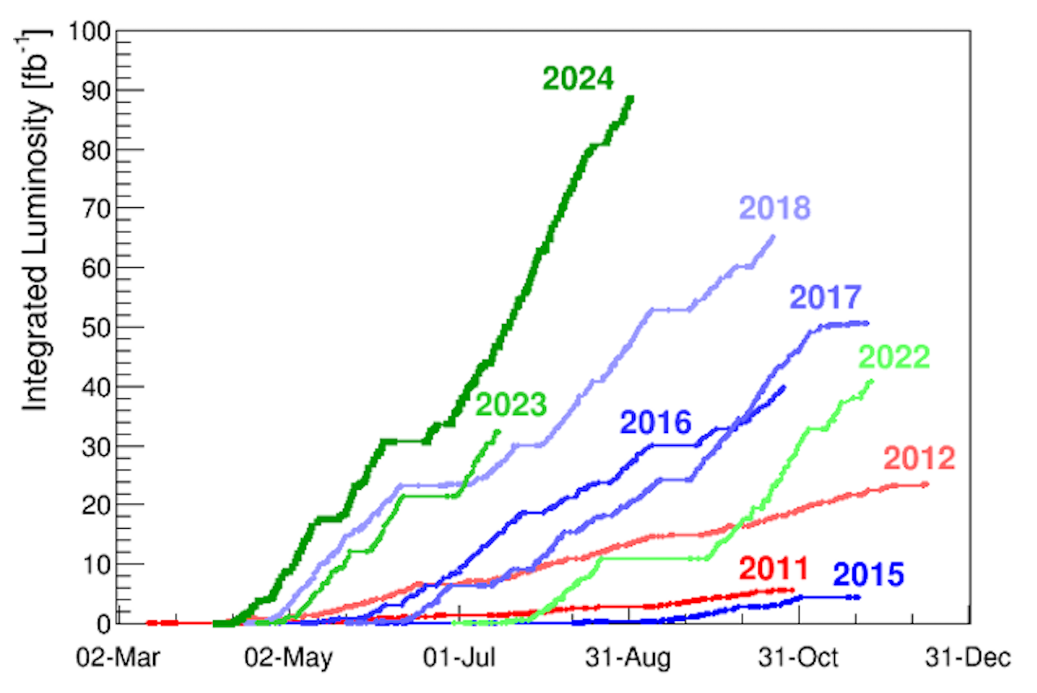
\includegraphics[width=0.75\textwidth]{Grafik.png}
\end{center}
Interpretieren Sie die Grafik unter Berücksichtigung folgender Fragen:
\begin{itemize}
    \item In welchem Jahr fanden die bisher meisten $pp$-Wechselwirkungen statt?
    \begin{answerbox}
        Da die Zahl der Wechselwirkungen proportional zur integrierten Luminosität ist, fanden im Jahr mit der größten erreichten integrierten Luminosität auch die meisten \(pp\)-Wechselwirkungen statt. Aus der Grafik sieht man, dass \(\textbf{2024}\) mit etwa \(90\,\mathrm{fb}^{-1}\) den größten Wert erreicht. Also fanden \textbf{2024} die meisten \(pp\)-Wechselwirkungen statt.
    \end{answerbox}
    \item Warum steigen die Verläufe nicht kontinuierlich an?
    \begin{answerbox}
        Die Verläufe steigen nur dann an, wenn der LHC tatsächlich Daten aufnimmt, also Protonenstrahlen kollidieren. Dazwischen gibt es Unterbrechungen, zum Beispiel durch technische Wartung, Maschinenstudien, das erneute Befüllen des Beschleunigers oder allgemein Phasen ohne Physikbetrieb. Deshalb entstehen abschnittsweise flache Bereiche und kein gleichmäßiger kontinuierlicher Anstieg.
    \end{answerbox}
    \item Könnte so ein Verlauf auch abfallen?
    \begin{answerbox}
        Nein. Die integrierte Luminosität ist ein über die Zeit aufsummierter Wert. Sie kann daher entweder konstant bleiben oder weiter ansteigen, aber nicht kleiner werden.
    \end{answerbox}
\end{itemize}
\end{enumerate}

\end{document}